%%% Group 4: Tahoe, Ksenia Sokolova, Xinmeng
%%% Computational Physics
%%% Spring, 2017

%%%%%%%%%%%%%%%%%%%%%%%%%%%%%%%%%%%%%%%%%%%%%%%%%%%%%%%%%%%%%%%%%%%%%%%%%%%%%%%%
%%% This code will develop a LaTeX'd writeup of the first group project
%%% assignment for PHYS566.
%%%%%%%%%%%%%%%%%%%%%%%%%%%%%%%%%%%%%%%%%%%%%%%%%%%%%%%%%%%%%%%%%%%%%%%%%%%%%%%%

% PACKAGES AND OTHER DOCUMENT CONFIGURATIONS
\documentclass[10pt]{article}
\usepackage[english]{babel}
\usepackage[utf8]{inputenc}
\usepackage{amsmath,amsfonts,amssymb}
\usepackage{graphicx,xcolor}
\usepackage{subfig}
\usepackage{booktabs}
\usepackage[left=2cm,%
right=2cm,%
top=2cm,%
bottom=2cm,%
headheight=11pt,%
letterpaper]{geometry}%
\usepackage{fancyhdr}
\pagestyle{fancy}
\lhead{\small\sffamily\bfseries\leftmark}%
\chead{}%
\rhead{\small\sffamily\bfseries\rightmark}
\renewcommand{\headrulewidth}{1pt}
\renewcommand{\footrulewidth}{1pt}
%\graphicspath{{}}

% Article Information
\title{Random Walks, the Diffusion Equation, and Cluster Growth}
\author{Tahoe Schrader, Ksenia Sokolova, Xinmeng \\PHYS566}
\date{}

% Begin writing document
\begin{document}
\maketitle

% Start with the abstract
\abstract{In this assignment we blah blah blah}

\section{Theory}
\label{sec:theory}

\subsection{Random Walks in 2D}
Mean and squared displacement
Distance from origin

\subsection{Diffusion Equations and the Finite Difference Form}
\label{sec:diffusionequation}
The diffusion equation in $1D$ is written,
\begin{equation}
  \label{eq:diffusioneqn}
  \frac{\partial\rho(x,t)}{\partial t} = D\nabla^2\rho(x,t),
\end{equation}
where $D$ is the diffusion constant. Equation~\ref{eq:diffusioneqn} is turned into an iterable form by noting: $\rho(x,t) = \rho(i\Delta x, n\Delta t) = \rho(i,n)$. This is the finite difference form\footnote{The finite difference form must be used because the diffusion equation is time dependent. Therefore, a relaxation method cannot be used.}.

After using the formal definition of derivatives and algebraically manipulating Equation~\ref{eq:diffusioneqn} in the finite difference form, we get
\begin{equation}
  \label{eq:diffusioneqn-iterable}
  \rho(i,n+1) = \rho(i,n) + \frac{D\Delta t}{\Delta x^2}\left(\rho(i+1,n) + \rho(i-1,n) - 2\rho(i,n)\right),
\end{equation}
where $\Delta t$ and $\Delta x$ are the step sizes in an iteration. This solution requires knowledge of initial conditions. We must assume that the $x$ displacement is known at times prior to and including $t_n = n\Delta t$. Two consecutive steps prior to the first unknown step is sufficient to solve such an equation.

We will use an initial density profile that is sharply peaked around $x=0$, but extends over a few grid sites to resemble a box. This is sufficient for generating the solution to the diffusion equation. Interestingly, after a couple iterations, the box profile will diffuse into a Gaussian normal distribution. The $1D$ Gaussian normal distribution has the form,
\begin{equation}
  \label{eq:gaussiandistribution}
  \rho(x,t) = \frac{1}{\sqrt{2\pi\sigma(t)^2}}\exp\left(-\frac{x^2}{2\sigma(t)^2}\right),
\end{equation}
where $\sigma(t) = \sqrt{2Dt}$.

The spatial expectation value, $\langle x(t)^2\rangle$, of Equation~\ref{eq:gaussiandistribution} is equal to $\sigma(t)^2$.
%%% NEED TO SHOW THIS IS TRUE. WILL PUT THAT PROOF HERE

\section{Computations}
\label{sec:computations}

\subsection{Random Walks in 2D}
\label{sec:computationsRandomWalk}
To code for the basic 2D walk, we assume that the probability to step in either direction left, right, up or down is the same. Then, for every step, we generate a random number. This is equivalent to drawing from Uniform (0,1). We assign every move to one of the segments of .25. If the random numbers falls within that value, we move in the assigned direction. The evidence for a successfully coded $2D$ walker program is given in Figure~\ref{fig:20steps} and \ref{fig:1000steps}.

\begin{figure}[!htb]
\minipage{0.5\textwidth}
  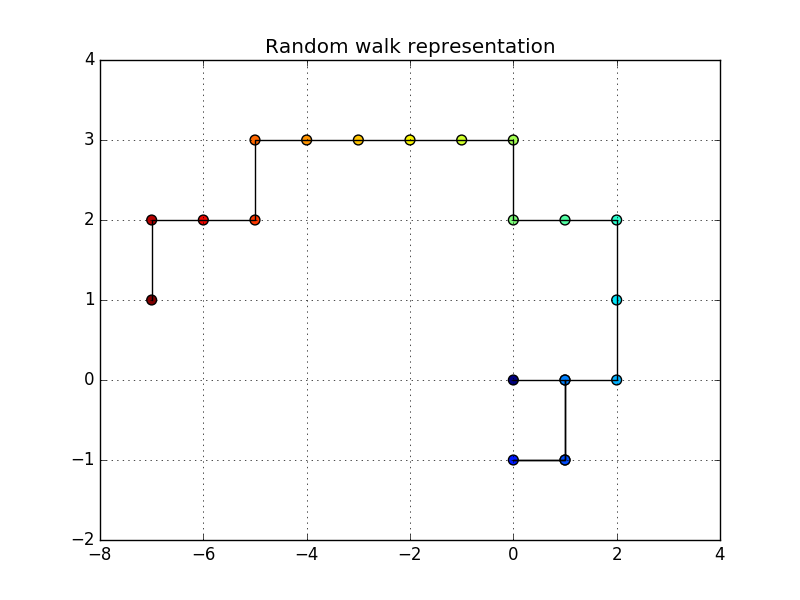
\includegraphics[width=\linewidth]{run20.png}
  \caption{20-step random walk}\label{fig:20steps}
\endminipage\hfill
\minipage{0.5\textwidth}
  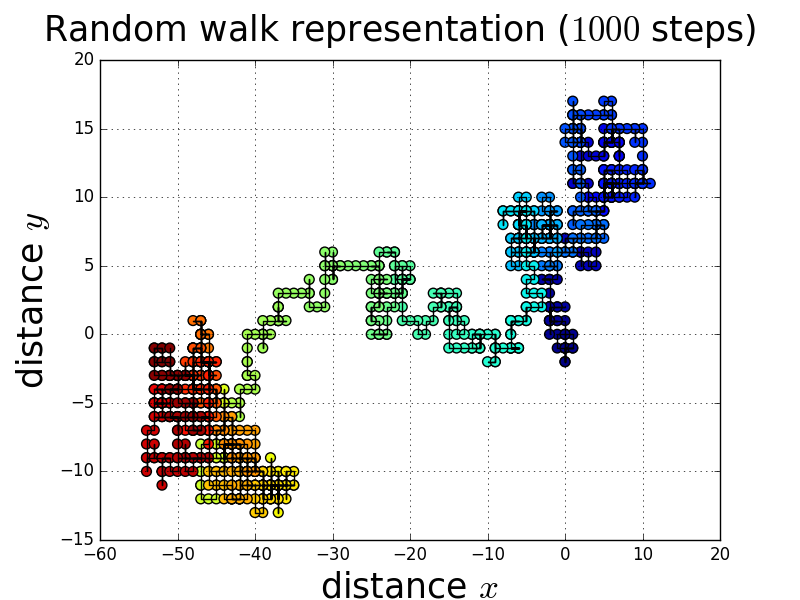
\includegraphics[width=\linewidth]{run1000.png}
  \caption{1000-step random walk}\label{fig:1000steps}
\endminipage\hfill
\end{figure}

\subsection{Diffusion of a Box Density Distribution}
\label{sec:diffusion-boxdensity}
Using the arguments in Section~\ref{sec:diffusionequation}, we solve the $1D$ Diffusion Equation over a period of time. Five different snapshots in time were then fit against Equation~\ref{eq:gaussiandistribution} to show a box shaped density will eventually diffuse into a Gaussian normal distribution.

%%% PUT THAT PLOT HERE

\end{document} % This ends our document

% INCOMPLETE
